
\section*{Appendix 1: Datasets Details}

\paragraph{PersonaBench.} 
PersonaBench~\cite{tan2025personabench}\footnote{\url{https://github.com/SalesforceAIResearch/personabench}} is a benchmark dataset designed to evaluate personalized retrieval grounded in user-specific contexts. It includes six users, each associated with a heterogeneous personal corpus composed of (i) conversations with friends (Conv.), (ii) dialogues with AI assistants (AI.), and (iii) e-commerce purchase histories (E-com.). For each user, 40--50 short and ambiguous natural language queries are provided (e.g., ``Do you know what my favorite color is?''), which require accurate grounding in the user’s prior behavior. This setup enables evaluation of models' ability to align with diverse personal semantics. Table~\ref{tab:personabench_stats} summarizes the query and corpus statistics across users.

\begin{table}[htbp]
    \centering
    \begin{tabular}{cccccccc}
    \toprule
    \textbf{User} & \textbf{Queries} & \textbf{Corpus} & \textbf{Conv.} & \textbf{AI} & \textbf{E-com.} \\
    \midrule
    1 & 48 & 110 & 84 & 23 & 3 \\
    2 & 43 & 90  & 78 & 8  & 4 \\
    3 & 42 & 64  & 51 & 12 & 1 \\
    4 & 46 & 85  & 71 & 14 & 0 \\
    5 & 44 & 84  & 59 & 21 & 4 \\
    6 & 40 & 94  & 79 & 14 & 1 \\
    \midrule
    \textbf{Sum} & 263 & 527 & 422 & 92 & 13 \\
    \textbf{Avg} & \textbf{43.83} & \textbf{87.83} & \textbf{70.33} & \textbf{15.33} & \textbf{2.17} \\
    \bottomrule
    \end{tabular}
    \caption{Statistics of the PersonaBench dataset across six users. The \textit{Corpus} is the sum of \textit{Conv.}, \textit{AI.}, and \textit{E-com.}.}
    \label{tab:personabench_stats}
\end{table}

\paragraph{LongMemEval.}
LongMemEval~\cite{wu2025longmemeval}\footnote{\url{https://github.com/xiaowu0162/LongMemEval}} is a benchmark designed to evaluate the long-term memory capabilities of large language models, particularly their ability to retrieve task-relevant information from extended user-specific corpora. Each instance in the dataset consists of a factual question paired with a synthetic memory corpus simulating historical user data. The dataset includes two settings: \textit{LongMemEval-s}, where each question is associated with approximately 50 memories, and \textit{LongMemEval-m}, where each corpus contains over 500 memories. In total, both settings consist of 500 questions, allowing evaluation of memory retrieval precision under varying context lengths. This benchmark enables controlled analysis of personalized retrieval performance under realistic long-context scenarios.

\begin{table}[htbp]
\centering
\begin{tabular}{lcc}
\toprule
\textbf{Statistic} & \textbf{LME-s} & \textbf{LME-m} \\
\midrule
Total Questions & 500 & 500 \\
Total Memory & 25,112 & 250,948 \\
Min Memory per Question & 39 & 501 \\
Max Memory per Question & 66 & 506 \\
Avg Memory per Question & \textbf{50.22} & \textbf{501.90} \\
\bottomrule
\end{tabular}
\caption{Statistics of the LongMemEval dataset (LME). Both LME-s and LME-m contain 500 questions, with different sizes of associated memory corpora.}
\label{tab:longmemeval_stats_vertical}
\end{table}


\section*{Appendix 2: Implement Details}
\subsection*{More Detailed Implement}
% \paragraph{Implement details.}
% To verify the robustness of our approach, all methods are evaluated under three retrieval backbones: \texttt{multi-qa-MiniLM-L6-cos-v1}\footnote{\url{https://huggingface.co/sentence-transformers/multi-qa-MiniLM-L6-cos-v1}}, \texttt{all-MiniLM-L6-v2}\footnote{\url{https://huggingface.co/sentence-transformers/all-MiniLM-L6-v2}}, and \texttt{bge-base-en-v1.5}\footnote{\url{https://huggingface.co/BAAI/bge-base-en-v1.5}}. For a fair comparison, all query expansions are generated using GPT-4o-mini~\cite{achiam2023gpt}. In our \textbf{PBR} framework, we set $k_1=5$,$m=5$, $\theta=0.75$, and $k_2=10$ across \textit{Perosnabench} and \textit{LongMemEval-s}. The larger $k_2=50$ is particularly suited for \textit{LongMemEval-m}, which contains richer user histories. More details are provided in Appendix 2.
\paragraph{Base Settings}:
% All retrieval experiments are performed on a single NVIDIA A100 80GB GPU under Ubuntu 22.04.  Query expansion is generated using GPT-4o-Mini with a temperature of 0. And each experiment we run 5 times.
All retrieval experiments are performed on an advanced GPU under Ubuntu 22.04.  Query expansion is generated using an advanced LLM with a temperature of 0. And each experiment we run 5 times.

\paragraph{Retrieval}: To verify the robustness of our approach, all methods are evaluated under three retrieval backbones: \texttt{multi-qa-MiniLM-L6-cos-v1}\footnote{\url{https://huggingface.co/sentence-transformers/multi-qa-MiniLM-L6-cos-v1}}, \texttt{all-MiniLM-L6-v2}\footnote{\url{https://huggingface.co/sentence-transformers/all-MiniLM-L6-v2}}, and \texttt{bge-base-en-v1.5}\footnote{\url{https://huggingface.co/BAAI/bge-base-en-v1.5}}. And FAISS to store the embedding vectors for efficient retrieval. For retrieval, we use Euclidean distance.


\subsection*{Prompt Templates for Query Expansion Methods}
% To ensure a fair and transparent comparison, we include below the full prompt templates used in each baseline and our proposed method. These prompts were carefully designed to align with the original paper. 
% For each method, we present the prompt in a structured \texttt{tcolorbox} format to highlight its content and style. These templates also reflect the diversity in expansion strategies, from shallow surface reformulations to deep context-grounded reasoning. We emphasize that all prompts were tested under identical generation settings to eliminate confounding factors from decoding behavior.

\subsection*{Prompt of Baselines}

To ensure a fair comparison, we implemented the prompt-based query expansion strategies of representative baseline methods.
% Each method employs a distinct prompting to zero-shot expand the query. 
These prompts were carefully designed to align with the original paper. 

\begin{tcolorbox}[colback=blue!5!white, colframe=blue!75!black, title=HyDE Prompt]
Please write a paragraph that answers the question.\\
\textbf{Question:} \texttt{\{query\}}\\
\textbf{Output:}
\end{tcolorbox}



\begin{tcolorbox}[colback=blue!5!white, colframe=blue!75!black, title=Query2Term Prompt]
Answer the following question:\\
\texttt{\{query\}}\\
Give the rationale before answering.
\end{tcolorbox}



\begin{tcolorbox}[colback=blue!5!white, colframe=blue!75!black, title=MILL Prompt]
What sub-queries should be searched to answer the following query?\\
Please generate 5 sub-queries with their related passages.\\
\textbf{Question:} \texttt{\{query\}}\\
You should only return a python list like:\\
\texttt{["query1 passage1", "query2 passage2", ..., "query5 passage5"]}\\
(no comments, no markdown) without any other words and explanation.
\end{tcolorbox}



\begin{tcolorbox}[colback=blue!5!white, colframe=blue!75!black, title=Chain-of-Thought Prompt]
Solve the question step-by-step.\\
\textbf{Question:} \texttt{\{query\}}
\end{tcolorbox}



\begin{tcolorbox}[colback=blue!5!white, colframe=blue!75!black, title=ThinkQE Prompt]
Given a question \texttt{'q'} and its possible answering passages (most are wrong):\\
1. \texttt{\{d1\}}; 2. \texttt{\{d2\}}; 3. \texttt{\{d3\}}; 4. \texttt{\{d4\}}; 5. \texttt{\{d5\}}\\
Please write a correct answering passage.\\
Use your own knowledge, not just the example passages!
\end{tcolorbox}


\subsection*{Prompt Design for Our Method}

% Our P-PRF involves a two-stage prompt design to jointly simulate user-specific expression  with utterance and reason. Below we present the two corresponding prompts:

\begin{tcolorbox}[colback=blue!5!white, colframe=blue!75!black, title=P-PRF-roughly]
You are to generate 10 natural candidate utterances the user might say, inspired by the dialogue history and the current question.

\textbf{Context}
\begin{itemize}
    \item \textbf{User dialogue history (for style imitation):} \texttt{\{history\}}
    \item \textbf{Current question (to inspire the utterances):} \texttt{\{query\}}
\end{itemize}

\textbf{Guidelines}
\begin{enumerate}
    \item Generate 10 fluent, natural utterances the user might plausibly say.
    \item Do \textbf{NOT} just paraphrase; include variations in tone, emphasis, or context.
    \item Each utterance should exceed 25 words.
    \item Reflect the style and tone consistent with the document.
    \item Return ONLY valid JSON in this format (no comments, no markdown):
    
    \texttt{
    \{
    "candidates": ["...", "...", "..."]
    \}
    }
\end{enumerate}
\end{tcolorbox}

\begin{tcolorbox}[colback=blue!5!white, colframe=blue!75!black, title=P-PRF-logically]
Solve the question step-by-step, inspired by the user dialogue history.

\textbf{Context}
\begin{itemize}
    \item \textbf{User dialogue history (for style imitation):} \texttt{\{history\}}
    \item \textbf{Current question (to inspire the reasoning):} \texttt{\{query\}}
\end{itemize}

\textbf{Output:} step-by-step explanation that maintains user-specific tone and reasoning patterns.
\end{tcolorbox}

Our P-PRF involves a two-stage prompt design to jointly simulate user-specific expression  with utterance and reason. 
% These two prompts work in tandem: P-PRF synthesizes diverse user-style-aligned utterances, while P-Anchor explicitly grounds these expansions via structured reasoning. Together, they allow the model to generate personalized and semantically anchored queries before retrieval.

\section*{Appendix 3: Extend Experiment}

\subsection*{Time Efficiency}

Table~\ref{tab:time_cost} reports the latency of each stage in the ThinkQE and PBR methods, measured in seconds. Both methods share similar preprocessing overheads during index construction and user information retrieval. PBR introduces an additional graph-building step (0.0008~s) to enhance personalized query expansion, which incurs negligible computational cost. The dominant latency for both methods arises from the query expansion generation stage, accounting for approximately 2.5--2.7~s, while the final retrieval stage remains lightweight. Overall, PBR achieves personalization with marginal additional latency about 0.18~s compared to ThinkQE.

\begin{table}[h]
\centering

\begin{tabular}{lcc}
\toprule
\textbf{Stage} & \textbf{ThinkQE} & \textbf{PBR} \\
\midrule
1. Build index & 0.0797 & 0.0797 \\
2. Build graph & -- & 0.0008 \\
3. Retrieval user info & 0.0043 & 0.0043 \\
4. Call API gen QE & 2.4999 & 2.6646 \\
5. Final retrieval & 0.0064 & 0.0167 \\
\bottomrule
\end{tabular}
\caption{Time latency of each stage in ThinkQE and PBR.}
\label{tab:time_cost}
\end{table}

\subsection*{Senitivity of $k_1$}
We further conducted a hyperparameter sensitivity analysis on the LongMemEval-S dataset, focusing on the impact of $k_1$, which controls the number of top-ranked candidates used in the retrieval of the P-PRF module. As shown in Table~\ref{tab:hyper_k1}, increasing $k_1$ from 3 to 10 consistently improves both {recall} and {ndcg} across all evaluation cutoffs. The gains are particularly evident at higher recall thresholds (e.g., R@5 increases from 0.8253 to 0.8401), indicating that a larger candidate pool allows the model to capture more diverse yet relevant context signals. We set $k_1=5$ as the default in the main experiments.

\begin{table}[htbp]
\setlength\tabcolsep{2.0pt}  %可以控制列间距
\centering
\caption{Hyperparameter sensitivity on the LongMemEval-S dataset under different values of $k_1$.}
\begin{tabular}{lcccccc}
\toprule
\textbf{$k_1$} & \textbf{R@1} & \textbf{N@1} & \textbf{R@3} & \textbf{N@3} & \textbf{R@5} & \textbf{N@5} \\
\midrule
3  & 0.2076 & 0.8258 & 0.7227 & 0.8402 & 0.8253 & 0.8519 \\
5  & 0.2100 & 0.8210 & 0.7279 & 0.8444 & 0.8282 & 0.8598 \\
10 & \textbf{0.2153} & \textbf{0.8305} & \textbf{0.7470} & \textbf{0.8504} & \textbf{0.8401} & \textbf{0.8661} \\
\bottomrule
\end{tabular}
\label{tab:hyper_k1}
\end{table}


\subsection*{Generation Performance}
To further evaluate the effect of personalized query expansion on generative outcomes, we conducted an additional experiment on the LongMemEval-S dataset under \texttt{multi-qa-MiniLM-L6-cos-v1} retriever. Following prior work on RAG evaluation~\cite{adlakha2024evaluating}, we adopt a subspan Exact Match (EM) metric to account for partial correctness in generative responses. As shown in Table~\ref{tab:gen_em}, PBR outperforms baseline query expansion approaches such as HyDE and CoT. Notably, PBR achieves the highest EM score of 42.6\%, surpassing the non-personalized CoT (41.0\%) and ThinkQE (41.8\%). These results demonstrate that integrating personalized query representation not only enhances retrieval accuracy but also yields measurable gains in final generation quality, confirming the cross-stage benefit of the proposed pre-retrieval personalization.

\begin{table}[htbp]
\centering
\caption{Generation performance (EM) on the LongMemEval-S dataset.}
\begin{tabular}{lc}
\toprule
\textbf{Method} & \textbf{EM (\%)} \\
\midrule
Base & 40.0 \\
HyDE & 41.4 \\
Query2Term & 40.2 \\
MILL & 40.8 \\
CoT & 41.0 \\
ThinkQE & 41.8 \\
PBR & \textbf{42.6} \\
\bottomrule
\end{tabular}
\label{tab:gen_em}
\end{table}




\begin{table*}[ht]
\centering
\resizebox{140mm}{!}{
\begin{tabular}{lcccccccc}
\toprule
& \multicolumn{2}{c}{\textbf{PBR}} 
& \multicolumn{2}{c}{\textbf{w/o P-Anchor}} 
& \multicolumn{2}{c}{\textbf{w/o P-PRF}} 
& \multicolumn{2}{c}{\textbf{w/o both}} \\
\cmidrule(lr){2-3} \cmidrule(lr){4-5} \cmidrule(lr){6-7} \cmidrule(lr){8-9}
Metrics & R@5 & N@5 & R@5 & N@5 & R@5 & N@5 & R@5 & N@5  \\
\midrule
\rowcolor{gray!15}
\multicolumn{9}{c}{\textit{multi-qa-MiniLM-L6-cos-v1}} \\
Overall & \textbf{0.5035} & \textbf{0.4201} & 0.4871 & 0.4100 & 0.3457 & 0.2877 & 0.4484 & 0.3669 \\
Basic information & \textbf{0.5091} & \textbf{0.3647} & 0.4833 & 0.3570 & 0.3318 & 0.2242 & 0.4515 & 0.3088 \\
Preference (hard) & 0.4049 & 0.4175 & \textbf{0.4390} & \textbf{0.4295} & 0.2683 & 0.2981 & 0.3659 & 0.3759 \\
Social & \textbf{0.5541} & \textbf{0.4914} & 0.5164 & 0.4529 & 0.4277 & 0.3851 & 0.4852 & 0.4356 \\
Preference (easy) & \textbf{0.5321} & \textbf{0.5129} & 0.5192 & 0.5160 & 0.3590 & 0.3414 & 0.4904 & 0.4582 \\
\midrule
\rowcolor{gray!15}
\multicolumn{9}{c}{\textit{all-MiniLM-L6-v2}}\\
Overall & \textbf{0.4516} & \textbf{0.3855} & 0.4382 & 0.3729 & 0.2860 & 0.2449 & 0.3783 & 0.3074 \\
Basic information  & \textbf{0.4515} & \textbf{0.3485} & 0.4379 & 0.3393 & 0.1985 & 0.1617 & 0.3515 & 0.2644 \\
Preference (hard)& \textbf{0.4341} & \textbf{0.4352} & 0.4244 & 0.4201 & 0.2878 & 0.2718 & 0.4000 & 0.3547 \\
Social & \textbf{0.4494} & \textbf{0.3777} & 0.4333 & 0.3639 & 0.4179 & 0.3387 & 0.3921 & 0.3048 \\
Preference (easy)& \textbf{0.4840} & \textbf{0.4800} & 0.4712 & 0.4587 & 0.3846 & 0.3634 & 0.4295 & 0.4199 \\
\midrule
\rowcolor{gray!15}
\multicolumn{9}{c}{\textit{BAAI/bge-base-en-v1.5}} \\ 
Overall & \textbf{0.4029} & \textbf{0.3402} & 0.3921 & 0.3256 & 0.2699 & 0.2214 & 0.3738 & 0.3015 \\
Basic information & \textbf{0.4121} & \textbf{0.3057} & 0.3970 & 0.2958 & 0.2576 & 0.1804 & 0.3970 & 0.2748 \\
Preference (hard) & 0.3707 & \textbf{0.3889} & \textbf{0.3902} & 0.3778 & 0.2146 & 0.2173 & 0.3268 & 0.3343 \\
Social& \textbf{0.3657} & \textbf{0.3089} & 0.3431 & 0.2822 & 0.3261 & 0.2816 & 0.3204 & 0.2799 \\
Preference (easy) & \textbf{0.4904} & \textbf{0.4734} & 0.4744 & 0.4582 & 0.2949 & 0.2785 & 0.4583 & 0.4065 \\
\midrule
\textbf{Average} & \textbf{0.4527} & \textbf{0.3819} & 0.4391 & 0.3695 & 0.3005 & 0.2513 & 0.4002 & 0.3253 \\
\bottomrule
\end{tabular}
}
\caption{Ablation study of PBR across different retrievers and subtasks.}
\label{tab:ablation_results}
\end{table*}

\begin{table*}[ht]
\centering

\resizebox{\textwidth}{!}{
\begin{tabular}{lcccccccccccc}
\toprule
\textbf{Dataset} 
& \multicolumn{6}{c}{\textbf{LongMenEval-s}} 
& \multicolumn{6}{c}{\textbf{LongMenEval-m}} \\
Metrics  & R@1 & N@1 & R@3 & N@3 & R@5 & N@5 & R@1 & N@1 & R@3 & N@3 & R@5 & N@5 \\
\midrule
\rowcolor{gray!15}
\multicolumn{13}{c}{\textit{multi-qa-MiniLM-L6-cos-v1}} \\
PBR              & \textbf{0.2100} & \textbf{0.8210} & \textbf{0.7279} & \textbf{0.8444} & \textbf{0.8282} & \textbf{0.8598} & \textbf{0.1217} & \textbf{0.5537} & \textbf{0.4320} & \textbf{0.5776} & \textbf{0.5537} & \textbf{0.6177} \\
w/o P-Anchor       & 0.2100 & 0.8129 & 0.7199 & 0.8385 & 0.8239 & 0.8420 & 0.1169 & 0.5456 & 0.4268 & 0.5623 & 0.5480 & 0.6127 \\
w/o P-PRF          & 0.1838 & 0.7566 & 0.6277 & 0.7540 & 0.7208 & 0.7739 & 0.1122 & 0.4893 & 0.3484 & 0.4961 & 0.4368 & 0.5303 \\
w/o Both         & 0.1885 & 0.7924 & 0.6730 & 0.8020 & 0.8067 & 0.8301 & 0.1098 & 0.5251 & 0.4057 & 0.5559 & 0.5394 & 0.6038 \\
\rowcolor{gray!15}
\multicolumn{13}{c}{\textit{all-MiniLM-L6-v2}}\\
PBR              & \textbf{0.2267} & \textbf{0.8592} & \textbf{0.7780} & \textbf{0.8754} & \textbf{0.8640} & \textbf{0.8902} & \textbf{0.1408} & \textbf{0.5800} & \textbf{0.4463} & \textbf{0.5949} & \textbf{0.5847} & \textbf{0.6424} \\
w/o P-Anchor       & 0.2191 & 0.8522 & 0.7628 & 0.8622 & 0.8511 & 0.8860 & 0.1360 & 0.5795 & 0.4435 & 0.5915 & 0.5819 & 0.6356 \\
w/o P-PRF          & 0.1957 & 0.7566 & 0.6563 & 0.7765 & 0.7589 & 0.8017 & 0.1217 & 0.4797 & 0.3628 & 0.4961 & 0.4678 & 0.5415 \\
w/o Both         & 0.2196 & 0.8234 & 0.7399 & 0.8477 & 0.8568 & 0.8731 & 0.1265 & 0.5322 & 0.4415 & 0.5857 & 0.5346 & 0.6191 \\
\midrule
\rowcolor{gray!15}
\multicolumn{13}{c}{\textit{BAAI/bge-base-en-v1.5}} \\ 
PBR              & \textbf{0.2315} & \textbf{0.8902} & \textbf{0.8138} & \textbf{0.9072} & \textbf{0.9045} & \textbf{0.9191} & \textbf{0.1408} & \textbf{0.6205} & \textbf{0.5489} & \textbf{0.6612} & \textbf{0.6874} & \textbf{0.7060} \\
w/o P-Anchor       & 0.2239 & 0.8850 & 0.8121 & 0.9037 & 0.8993 & 0.9154 & 0.1304 & 0.6125 & 0.5322 & 0.6579 & 0.6721 & 0.7007 \\
w/o P-PRF          & 0.2029 & 0.8234 & 0.7446 & 0.8517 & 0.8449 & 0.8704 & 0.1002 & 0.5298 & 0.4344 & 0.5698 & 0.5680 & 0.6125 \\
w/o Both         & 0.2267 & 0.8616 & 0.7900 & 0.8863 & 0.8926 & 0.9007 & 0.1217 & 0.5943 & 0.5322 & 0.6605 & 0.6444 & 0.6929 \\
\bottomrule
\end{tabular}
}
\caption{Ablation results of PBR on LongMenEval-s and LongMenEval-m datasets.}
\label{tab:ablation_longmen}
\end{table*}


\subsection*{Ablation Study in Two Datasets}
\paragraph{Complementary Ablation Insights.}  
Across both the retrieval backbones and datasets, we observe a \textit{consistent performance drop when either component (P-Anchor or P-PRF) is removed}, confirming their complementary contributions to the overall effectiveness of the PBR framework.

First, \textbf{removing P-PRF leads to the most significant degradation}, especially on more complex queries such as \texttt{Preference (hard)} and datasets like LongMenEval-m, where user intent is more nuanced. For example, on \texttt{multi-qa-MiniLM} in Table~\ref{tab:ablation_results}, R@5 drops from 0.5035 to 0.3457 without P-PRF, and similarly in Table~\ref{tab:ablation_longmen}, LongMenEval-s sees a drop in R@3 from 0.7780 to 0.6563 without P-PRF. This highlights the \textit{critical role of user-aware pseudo relevance feedback in capturing latent intent}.

Second, \textbf{removing P-Anchor has a more moderate but consistent impact}, especially in tasks requiring robust grounding of queries within diverse semantic corpora (e.g., \texttt{Social} and \texttt{Preference (easy)}). This suggests that \textit{style-consistent anchoring helps stabilize query representations}, particularly when user content is lexically varied.

Finally, the combination of removing both components consistently results in a \textbf{further drop}, but not always the worst performance. This indicates a certain degree of \textit{redundancy or shared effect between P-Anchor and P-PRF}, suggesting that while they operate on different principles (style anchoring vs. semantic feedback), they jointly reinforce personalized query understanding. On average (last row, Table~\ref{tab:ablation_results}), the full PBR outperforms the no-component baseline by \textbf{+13.1\% R@5} and \textbf{+17.4\% N@5}.


\subsection*{Effectiveness of P-PRF in Two Datasets}

\begin{figure*}[ht]
    \centering
    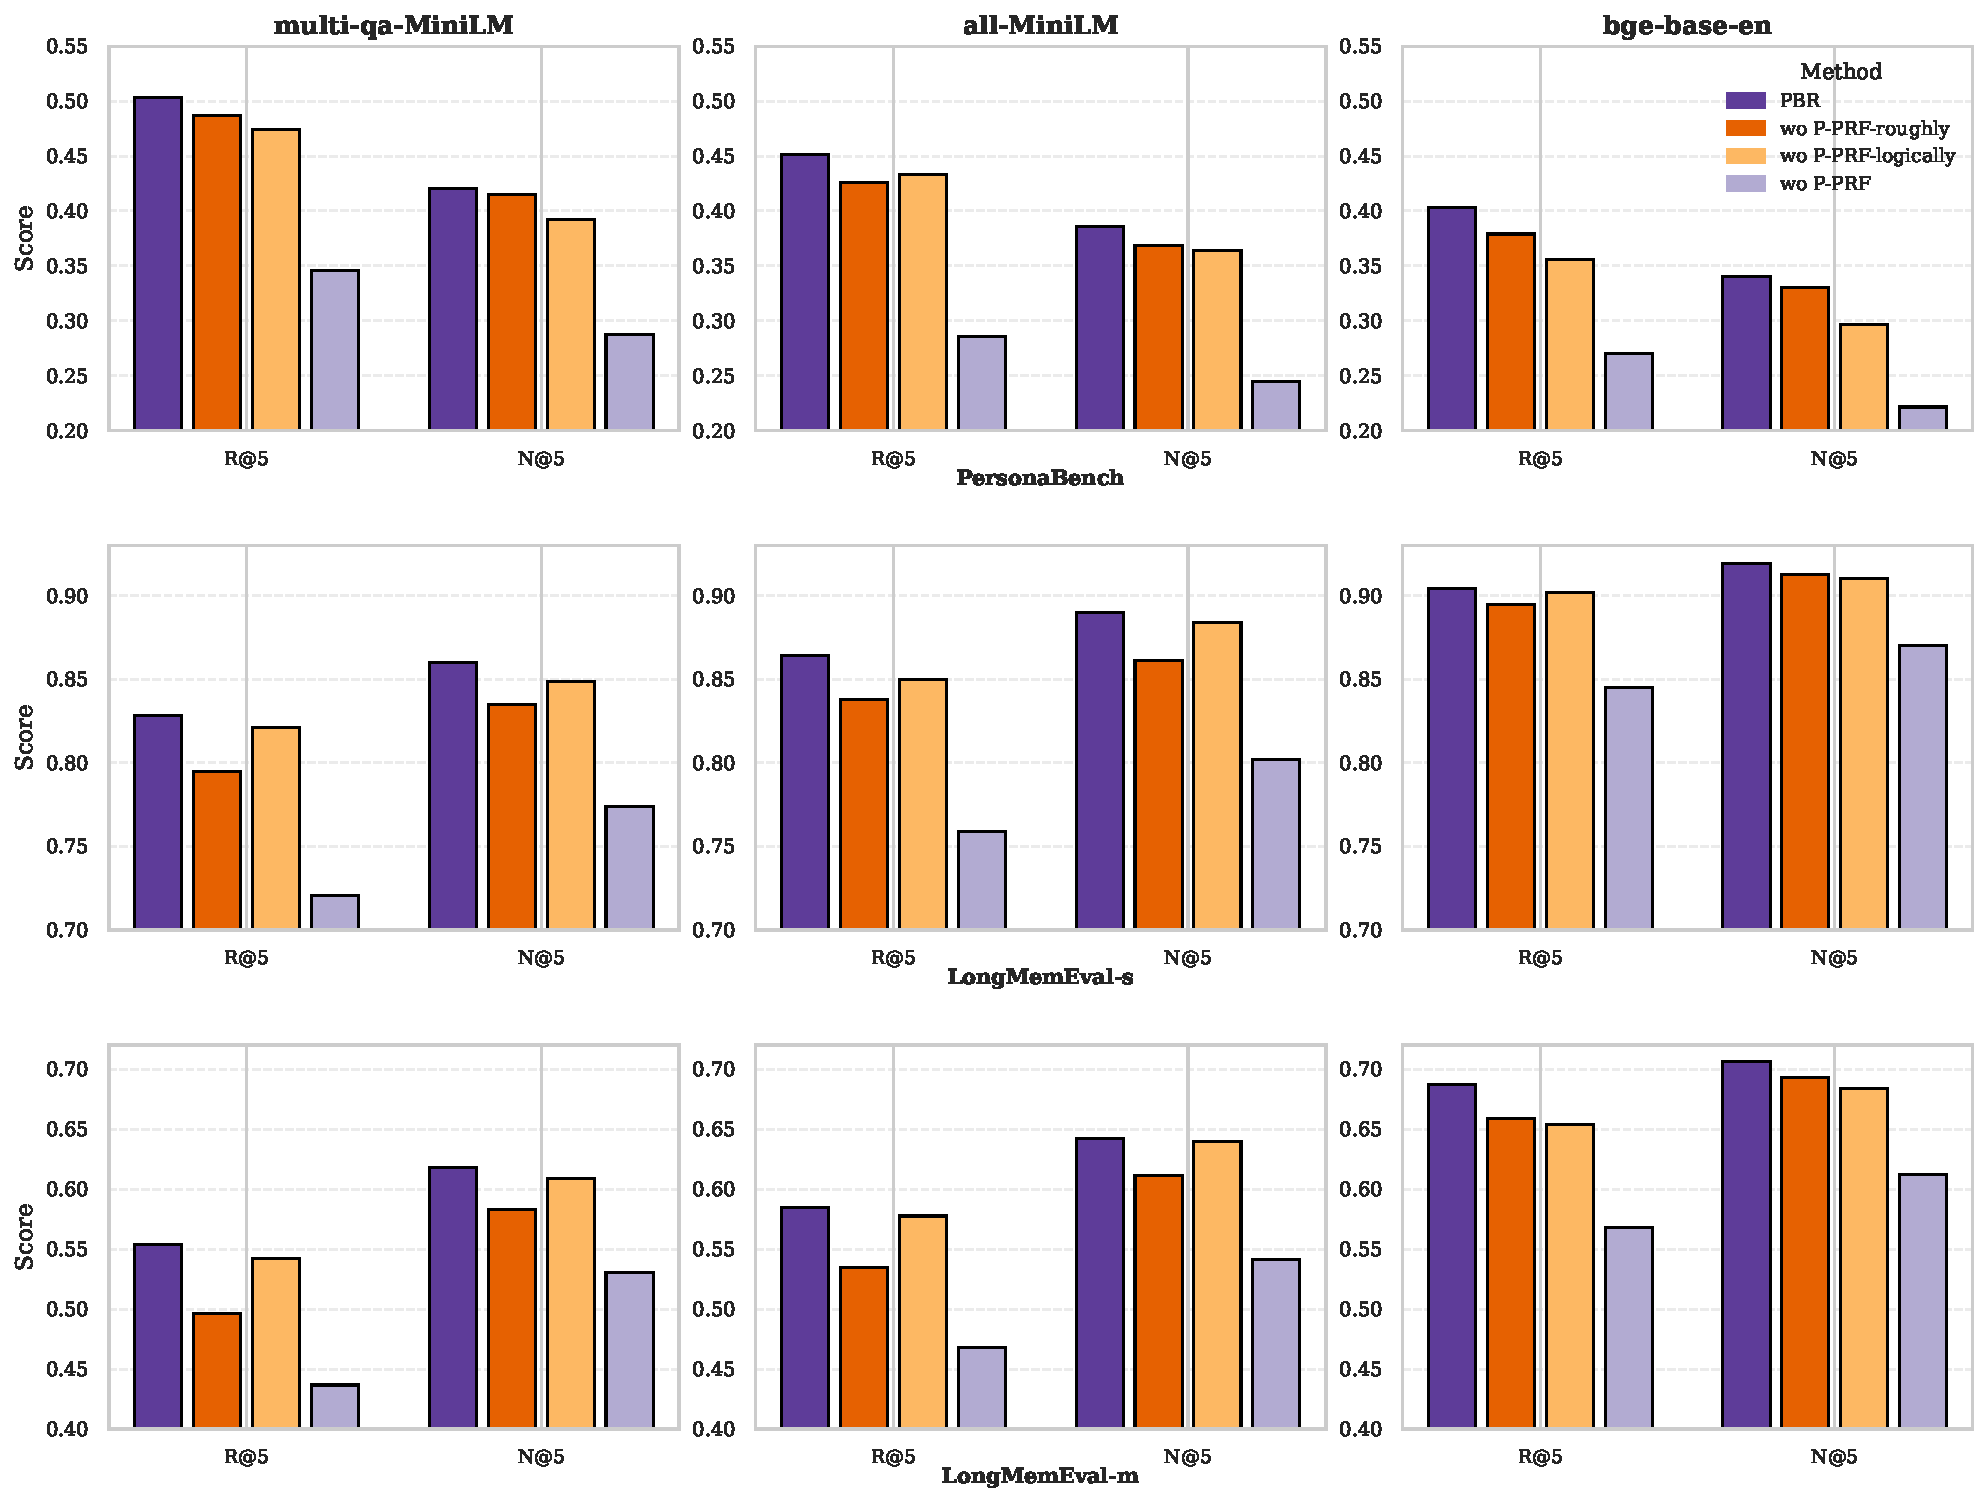
\includegraphics[width=0.98\linewidth]{figure/3x3_dataset_comparison.pdf}
    \caption{%
        Overall performance in \textit{Personabench} comparison across three ablation retrieval modes. 
    }
    \label{fig:pprf-ablation-all}
    \vspace{-10pt}
\end{figure*}


\paragraph{Visualization-based Analysis.} 
Figure~\ref{fig:pprf-ablation-all} presents a comparative bar plot of PBR and its ablated variants across three retrievers (multi-qa-MiniLM, all-MiniLM, bge-base-en) and three evaluation datasets (PersonaBench, LongMenEval-s, LongMenEval-m). Each subplot reports the R@5 and N@5 metrics, offering insight into both retrieval recall and ranking quality.

\textbf{(1) On \textit{PersonaBench}}, PBR consistently outperforms all variants across all retrievers. Notably, the drop in N@5 when removing P-PRF is more severe than the drop in R@5, indicating that pseudo-relevance feedback contributes more to fine-grained ranking alignment than coarse recall.

\textbf{(2) On \textit{LongMenEval-s}}, where queries are more succinct, the gap between PBR and its variants becomes more pronounced, especially under bge-base-en. This suggests that PRF-based refinements are crucial for handling underspecified queries by injecting user-grounded semantics into the expansion.

\textbf{(3) On \textit{LongMenEval-m}}, the performance degradation from removing P-PRF is still significant but relatively less than in LongMenEval-s. This is likely due to longer query inputs providing stronger initial signals, slightly compensating for the lack of PRF. However, the logical and rough removal of PRF still lags behind full PBR, validating the importance of structurally grounded expansion paths.

Overall, the visual analysis confirms the complementary roles of anchor-based grounding and pseudo-feedback refinement in boosting personalized retrieval quality across varied retriever and dataset settings.